\newcommand{\textretrieval}{\preprintonly{textretrieval-001}%
    \finalonly{textretrieval-001}%
    \submissiononly{moocname1-00X}}

\newcommand{\sustain}{\preprintonly{sustain-001}%
    \finalonly{sustain-001}%
    \submissiononly{moocname2-00X}}

\newcommand{\UIUC}{\preprintonly{UIUC}%
    \finalonly{UIUC}%
    \submissiononly{(redacted University)}}

\section{Results}
To qualitatively evaluate our model, we can look at the latent state
representations we learn by fitting the model to some MOOC log data. We can
also inspect the transition matrix between the latent states discovered by
the model.

Specifically, we look at the MOOC logs associated with two different
Coursera MOOCs offered by \UIUC{}: \textretrieval{} and \sustain{}.  The
\textretrieval{} MOOC represents a highly technical computer science course,
where the \sustain{} MOOC is more representative of a humanities course. We
picked these two MOOCs because of their vastly different content domains.
Table~\ref{table:datasets} summarizes the two datasets we extracted from
the MOOCs.

\begin{table}
  \begin{center}
    \begin{tabular}{rrrr}
      \textbf{MOOC} & \textbf{Students} & \textbf{Sequences} & \textbf{Avg.
      $|\mathbf{s}|$}\\\hline
      \textretrieval{} & 18,941 & 85,240 & 7.31\\
      \sustain{} & 85,240 & 231,881 & 15.4
    \end{tabular}
    \caption{Statistics about the sequences extracted from the two MOOCs.}
    \label{table:datasets}
  \end{center}
\end{table}

\subsection{Latent State Representations}
First, we fit a 6-state TL-HMM to the \textretrieval{} sequence dataset and
show some of the latent state representations we find. We used the
following ten actions as our action set $\mathbf{A}$:
\begin{enumerate*}[label=(\arabic*)]
  \item quiz start,
  \item quiz submit,
  \item wiki (course material),
  \item forum list (view the list of all forums),
  \item forum thread list (view the list of all threads in a specific
    forum),
  \item forum thread view (view the list of posts within a specific
    thread),
  \item forum search (a search query issued against the forum),
  \item forum post thread (a new thread was posted),
  \item forum post reply (a new post was created within an existing
    thread), and
  \item view lecture (defined as either streaming or downloading a lecture
    video).
\end{enumerate*}

To visualize these Markov models that represent our latent states, we plot
them as a directed graph where we set the size of a node to be proportional
to its personalized Pagerank score~\cite{Page:1999:PageRank, Jeh:2003:WWW}
where the personalization vector is the initial state distribution for the
Markov model. We let the thickness of a directed edge $(u, v)$ reflect the
probability of taking that edge given that a random walk is currently at
note $u$ (as indicated by the transition matrix). The plots were created
using python-igraph\footnote{\url{http://igraph.org/python/}}.

\begin{figure*}
  \centering
  \begin{subfigure}[t]{0.5\textwidth}
    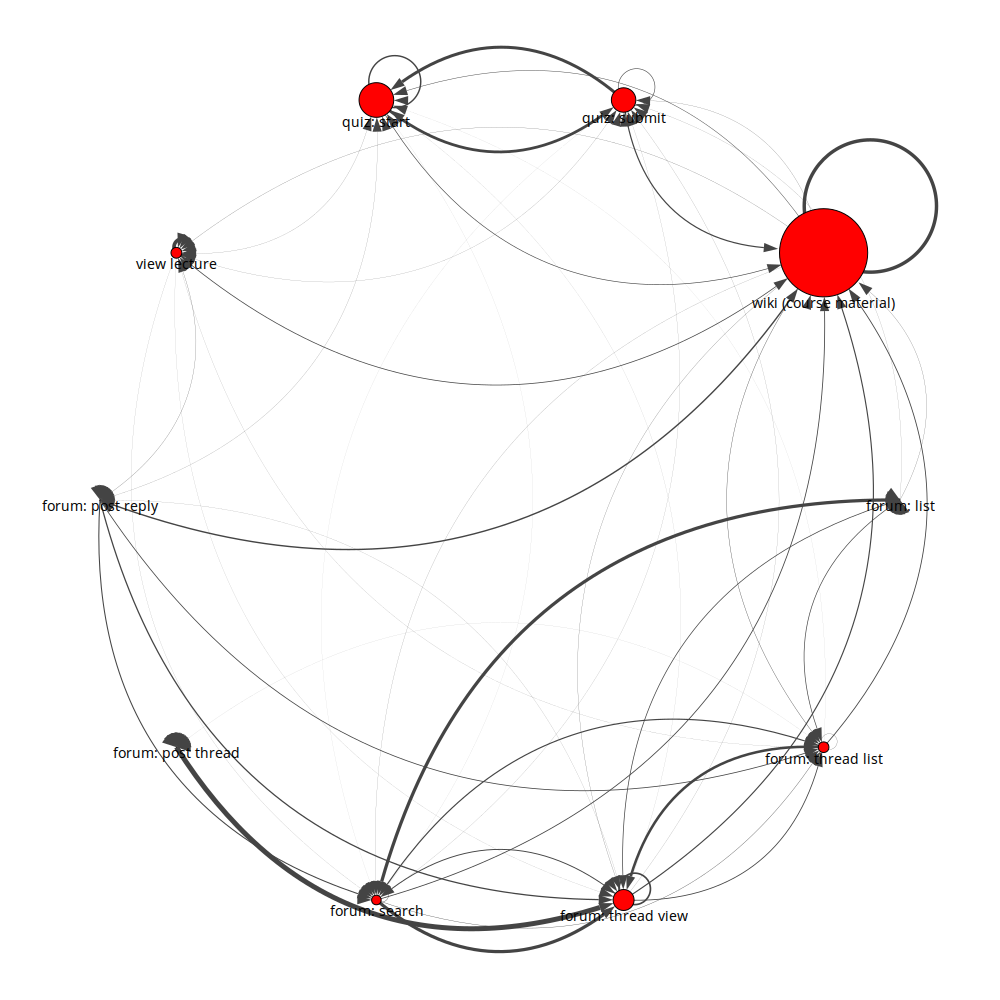
\includegraphics[width=\textwidth]{figures/text-6state/state0.png}
    \caption{An example ``quiz taking'' state.}
    \label{fig:practice-quiz-state}
  \end{subfigure}%
  \begin{subfigure}[t]{0.5\textwidth}
    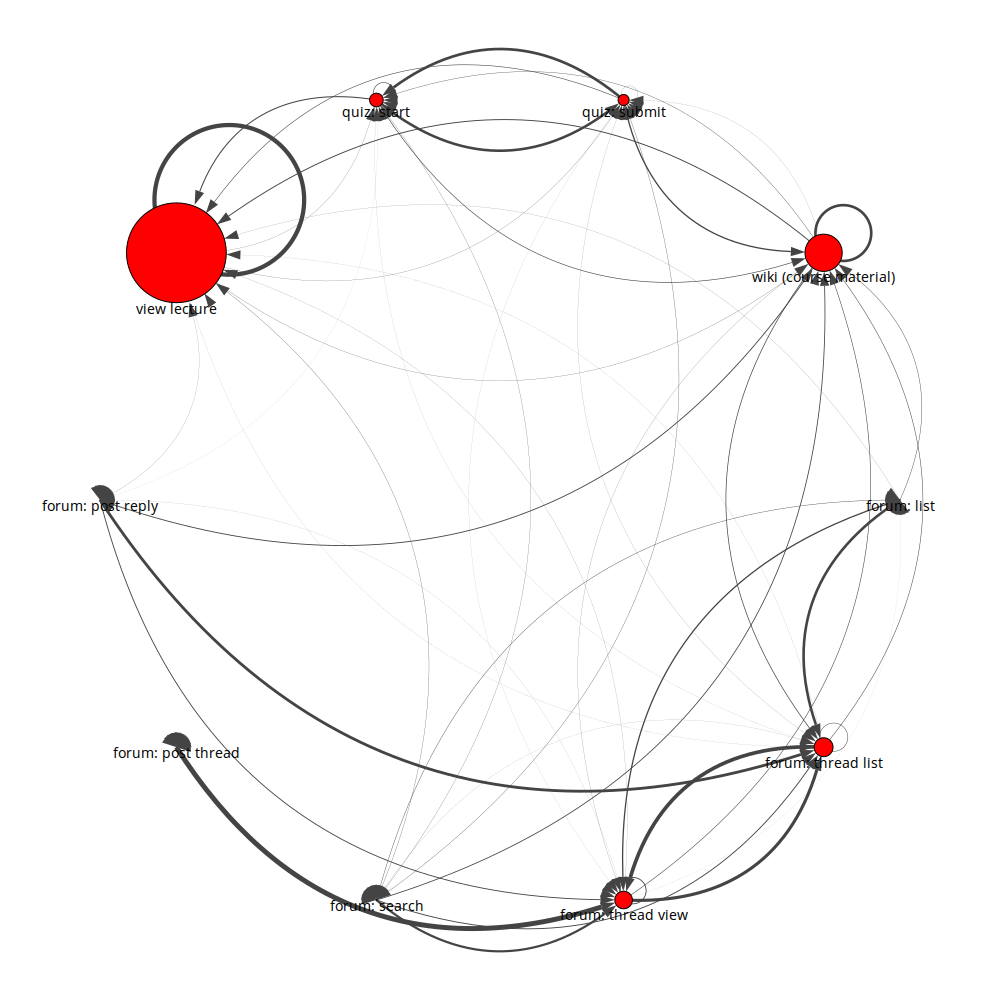
\includegraphics[width=\textwidth]{figures/text-6state/state1.png}
    \caption{An example ``lecture viewing'' state.}
    \label{fig:lecture-viewing-state}
  \end{subfigure}
  \caption{Two example states found by the 6-state TL-HMM.}
  \label{fig:states}
\end{figure*}

Figure~\ref{fig:states} includes two such representations we learned. The
first corresponds to a ``quiz taking'' state whereas the second corresponds
to a ``lecture viewing'' state. Clearly, our unsupervised method can
uncover states that do indeed correspond to student behavior modes that we
would expect to find a priori.

We also argue that it is important that the latent state representation be
a Markov model rather than just a discrete distribution over actions in
$\mathbf{A}$ (as would be the case for a traditional single-layer HMM). We
can observe why if we take a closer look at each of the two latent state
representations in Figure~\ref{fig:states} and look at their forum
component (bottom right). We can see that the relative probability of the
forum activities is roughly the same between these states, but the
\emph{transitions} are quite different. In
Figure~\ref{fig:practice-quiz-state} we have a relatively low probability
of walking from the ``forum thread view'' action back to the ``forum thread
list'' action, but in Figure~\ref{fig:lecture-viewing-state} we actually
observe a very strong link in this direction. This difference highlights an
important distinction between these two latent states: in the first you are
more likely to visit the forum \emph{looking for a particular post}, where
in the second you are more likely to visit the forum \emph{to browse
existing posts}. Thus, capturing the action transition matrix within a
latent state is important for capturing detailed insights involving bigrams
of actions.

% highlight interesting latent states discovered; make arguments that
% motivate why it's useful to have a Markov model as the latent state
% representation (capturing transitions between actions is useful and
% more meaningful than just using a discrete distribution as the latent
% state representation); show how the learned state representations differ
% between the two MOOCs

\subsection{Varying the Number of Latent States}
% show what happens as we vary k (particularly interesting to see 2 -> 3
% hidden state change, as the forum "topic" appears suddenly); argue that
% this allows the model to capture behavior patterns at different levels of
% granularity

\subsection{Transitions Between Latent States}
% using k=6, show that we can uncover interesting patterns in how students
% transition between the different latent states; argue that this discovery
% is interesting and unique to our formulation and could not be discovered
% before
